\chapter{Design\label{chap:design}}
In this chapter, there is a discussion about the software that was created during this project, its elements and how they interconnect. Design charts showcasing high-level overview are also included, alongside with the architecture split onto layers - which are loosely coupled with each other. Finally, the presentation of novel approaches such as verifying the authenticity of the connecting clients, the data model stored on the blockchain and how the connection is secured from man-in-the-middle attacks through TLS encryption is shown.

\section{Architecture}\label{sec:arch}
This section includes the diagram of the system and two sample workflows demonstrating how packets are flowing through the framework.
\subsection{Overview}
\begin{figure}[h]
    \centering
    \makebox[\textwidth][c]{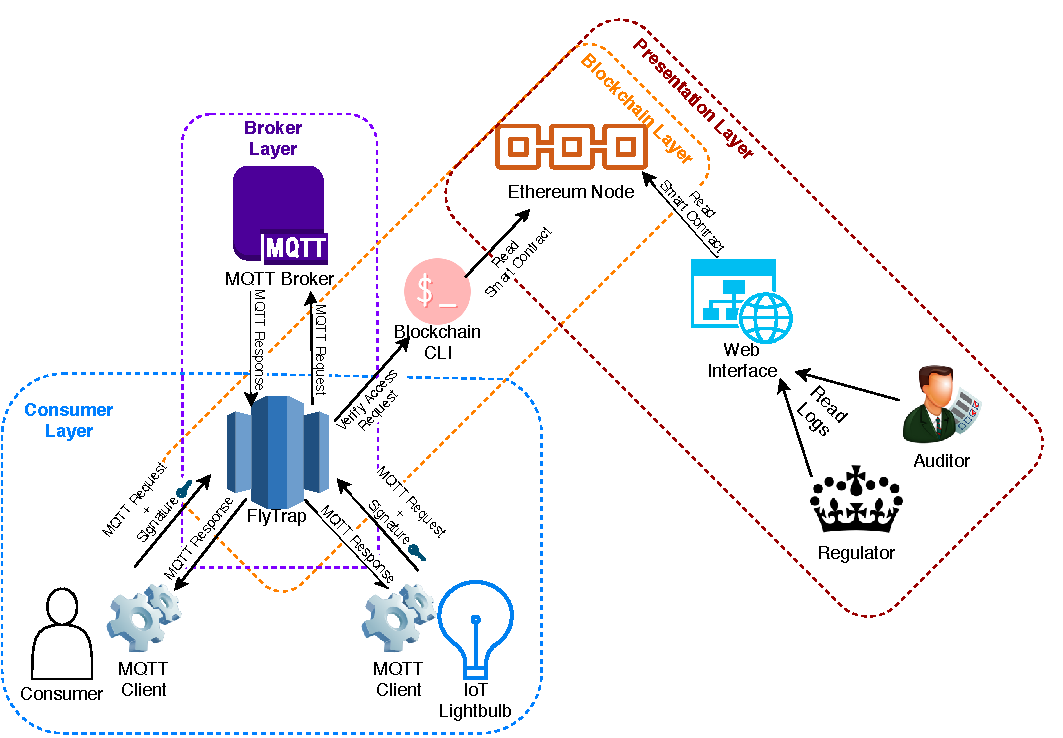
\includegraphics[width=1.2\textwidth]{flytrap}}
    \caption{FlyTrap high-level architecture overview}
    \label{fig:flytrap}
\end{figure}
Figure \ref{fig:flytrap} presents an overview of the system, decomposing it into four layers, each responsible for a different part of the framework. It also demonstrates how those layers are coupled and the direction of data flowing between them.

The four layers are as follows:
\begin{description}
    \item[Consumer Layer] - Responsible for interacting with end-devices. To them, FlyTrap should be indistinguishable from a normal MQTT broker and thus accepts/responds with MQTT v5.0 compliant TCP/TLS packets. 
    \item[Consumer Layer] - Here FlyTrap acts like a client for the MQTT Broker. Similar to the Consumer Layer, all packets sent by FlyTrap need to be compliant with the MQTT standard in order to receive valid responses from the broker. In this situation, the utilised broker is not relevant - as long as it implements the standard and responds with standarised MQTT packets.
    \item[Blockchain Layer] - Here FlyTrap performs communication with the Ethereum node through a separate CLI. FlyTrap is capable of either reading past contracts/transactions or submitting new ones. This also provides an opportunity to amend the state of the blockchain (such as access control lists) - given the private master key has remained secret.
    \item[Presentation Layer] - Used by FlyTrap's end-users to access an overview of the state of the blockchain in a user-friendly way, easily extracting most relevant information such as reports from sensistive topics or audit trail for major operations on the chain.
\end{description}


\subsection{Sample Successful PUBLISH Workflow}
To provide further context, Figure~\ref{fig:workflow_success} provides an example process in which a client wants to publish a message to the broker and is successful in doing so. The diagram shows step-by-step the logic performed at each stage of the connection, until the client receives the response. Each step is annotated with either \textbf{BL} - Blockchain Layer, \textbf{CL} - Consumer Layer or \textbf{ML} - MQTT Broker Layer to signify the layer in which this step takes places.
\begin{figure}[h]
    \centering
    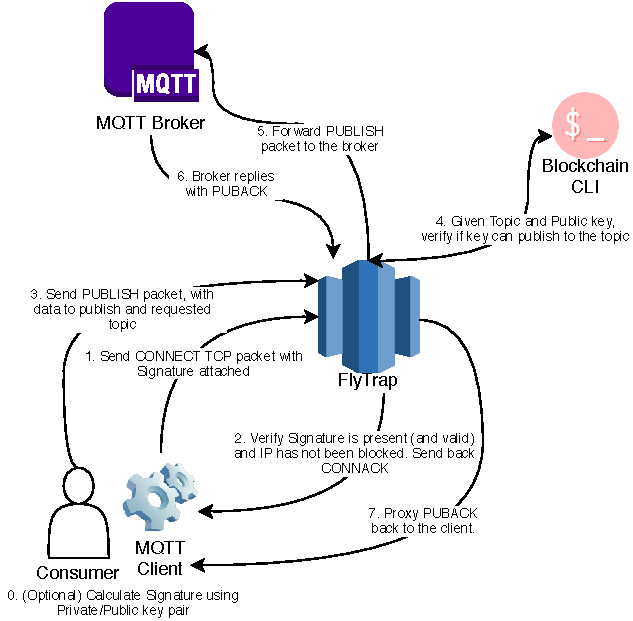
\includegraphics[width=0.8\textwidth]{workflow_success}
    \caption{Example successful workflow to publish a message on the broker through FlyTrap.}
    \label{fig:workflow_success}
\end{figure}

Explanation of each step:
\begin{enumerate}\addtocounter{enumi}{-1}
    \item Marked as optional since each client can accept a pre-computed signature, which can be loaded onto the device; this can be helpful for situations where there is not enough computational power for calculations. (\textbf{CL})
    \item Client sends CONNECT packet, including signature + public key in the optional fields of MQTT message. (\textbf{CL})
    \item FlyTrap extracts the signature from the optional field and then verify its integrity. It also checks if the client has not been attempting many unsuccessful connections.\footnote{By looking up in-memory dictionary, see Section \ref{sec:ddos} for details.} Finally, FlyTrap responds with CONNACK, signalling to the client that it may now submit relevant payload packets. If the integrity check has failed, CONNACK would also have a flipped flag indicating rejected connection and cease further communication. (\textbf{CL})
    \item Client now forwards the relevant PUBLISH/SUBSCRIBE packet to FlyTrap (as it still believes that it is a regular MQTT broker). (\textbf{CL})
    \item FlyTrap now extracts the requested topic from the MQTT packet and communicate with the blockchain, presenting Public Key and requested topic to verify whether data can be accessed. For this example, the access check was successful. (\textbf{BL})
    \item FlyTrap proxies (unchanged) PUBLISH packet to the actual MQTT broker. (\textbf{ML})
    \item MQTT broker now responds with PUBACK, indicating successful PUBLISH. (\textbf{ML})
    \item Finally, FlyTrap proxies the same PUBACK packet back to the initial client to let them know that the operation was successful - and at the end, gracefully terminate the connection. (\textbf{CL})
\end{enumerate}

\subsection{Sample Failed PUBLISH Workflow}
In this workflow we demonstrate a similar operation, but with the difference being that this time the connection is not allowed, as the presented Public Key is not allowed to publish information on the given topic. For the sake of brevity, steps 0-3 are skipped - as they are identical to the successful scenario.

Below you can find extra details on each step outlined by Figure~\ref{fig:workflow_fail}:
\begin{enumerate}\addtocounter{enumi}{4}
    \item[4-5.] Having verified the authenticity of the Public Key, FlyTrap again tries to verify with the Smart Contract whether the client can access the topic. This time though, the response is negative, and the client is not allowed to publish on the requested topic.
    \item FlyTrap sends PUBACK back to the client, setting reason code\footnote{https://docs.oasis-open.org/mqtt/mqtt/v5.0/os/mqtt-v5.0-os.html\#\_Toc3901124} to "Not authorised", at the same time terminating the connection with the client. To client, the situation is to that occurring when an invalid username/password is set to a vanilla MQTT broker.
    \item Framework verifies with the cached values to check if the originating IP has not exceeded the maximum number of allowed tries. If it did, it could place it on a blacklist, and every subsequent connection is denied for the specified time. In this example, that is 5 minutes. This step is optional.
    \item If the ban happens, FlyTrap also registeres a new transaction on the blockchain to persistently log this event to check potential attack spikes or generate reports w.r.t.  captured data. This step is also optional.
\end{enumerate}

Note: as can be seen from Figure~\ref{fig:workflow_fail}, the MQTT Broker is never connected to nor contacted with the potentially malicious message. FlyTrap rejects the message and forbids the connection. 
\begin{figure}[h]
    \centering
    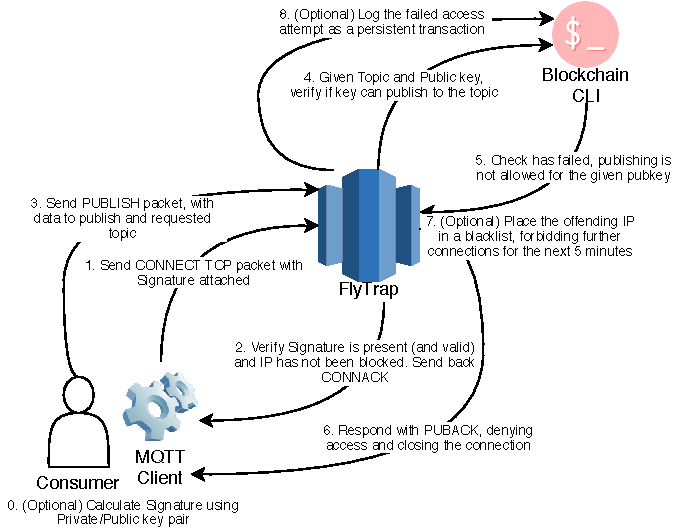
\includegraphics[width=0.9\textwidth]{workflow_fail}
    \caption{Example failed workflow to publish a message on the broker through FlyTrap}
    \label{fig:workflow_fail}
\end{figure}

\section{Layer Decomposition}
This section overviews each of the layers discussed in Section \ref{sec:arch} and as shown in Figure \ref{fig:flytrap}.
\subsection{Consumer Layer}
This part of the framework handles all connections between clients attempting to PUBLISH or SUBSCRIBE to data. To them, FlyTrap should be indistinguishable from a vanilla MQTT broker, which should be accepting all regular MQTT payloads. Although the MQTT client produced in this project can connect with every MQTT Broker, a specific client is required for connection with FlyTrap (due to extra authentication fields) - which is further explained in the section below. Moreover, an approach of identifying whether the client holds a Private Key for the presented Public Key is here explained. 
\subsubsection{MQTT Client}
FlyTrap makes use of the User Properties\footnote{https://docs.oasis-open.org/mqtt/mqtt/v5.0/os/mqtt-v5.0-os.html\#\_Toc3901068} introduced in MQTT v5.0, allowing clients to include key-value pairs in the MQTT packets, which then can be utilised by the brokers (or other middleware). That is also where the signature and public key is being placed by the client when attempting connection with FlyTrap - and that is also the need for a custom client since regular clients are not capable of producing highly specialised signatures to connect with Ethereum blockchain.

It is important to point out that the client is only slightly altered to provide (and compute if needed) the signature from a public/private key pair. It is not a critical part of FlyTrap, as any client capable of setting User Properties for an MQTT message would be sufficient, though, for the purposes of this dissertation, a custom implementation has also been designed and included. The User Properties are also ignored by regular brokers.

FlyTrap only expects two custom properties, set on the CONNECT message (meaning that other packets, such as PUBLISH or SUBSCRIBE remain untouched). The properties are: plain-text public key mapped to key ``pub'' and public key signed with the private-key mapped to ``sig'' (as can be seen in Figure~\ref{fig:sign}).

\subsubsection{Authenticity of Public Keys}
Public Keys from the Ethereum wallet are used as an identifier when determining whether a client can access a given resource or not. Public keys, by definition are, public, meaning that anyone could impersonate legitimate holders of the public/private key pairs. This calls for an approach similar to the Certificate Authority problem when attempting encrypted HTTPS connections. Unfortunately, FlyTrap cannot expect every IoT device to have its own set of certificates, which would then need to be trusted by the framework in order to become recognisable - as those devices are often of limited storage and power.

In order to solve the problem of establishing whether the person presenting a public key also holds a corresponding key, a novel authentication method utilising signatures is used. Figures \ref{fig:sign} and \ref{fig:verify} outline client-side and FlyTrap side of the signing/verification process.

\begin{figure}[h]
    \centering
    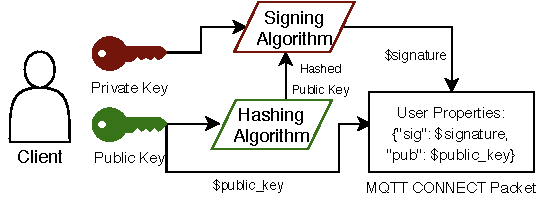
\includegraphics[width=0.8\textwidth]{sign}
    \caption{Client signing public key and attaching it to the message.}
    \label{fig:sign}
\end{figure}

Figure \ref{fig:sign} shows how a client - in possession of public/private key pair produces a signature which then is attached to the final MQTT CONNECT packet. First, it hashes the public key using Keccak-256 algorithm \cite{bertoni2009keccak} (commonly used in Ethereum, e.g. for block hashes), then it uses the private key to sign this hash and attaches the obtained signature to the user properties part of the MQTT CONNECT message. A plain-text version of the public key is also attached in another field. Ethereum signatures are created by signing arbitrary bytes through a generated private key - which then can only be verified using the corresponding public key. It is also possible to extract signed bytes from the same signature in the process.

\begin{figure}[h]
    \centering
     \makebox[\textwidth][c]{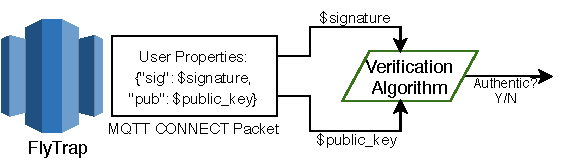
\includegraphics[width=1.1\textwidth]{verify}}
    \caption{FlyTrap verifying the signature.}
    \label{fig:verify}
\end{figure}

Then, as per Figure~\ref{fig:verify}, FlyTrap receives the CONNECT packet and extracts both the signature \& public key from the message. As the corresponding private key for the public key was used to produce the signature, the framework verifies this through Verification Algorithm\footnote{\label{fot1}Here, it is an Elliptic Curve Digital Signature Verification}. The output is a binary yes/no value - determining whether the public key was used to create the signature - along with the signed value (in this case, hashed public key) by the client. Then, the framework can verify whether signature was indeed created with the private key corresponding to the attached public key and (by hashing it again) compare the extracted value with the attached public key. This gives a definite answer that the person presenting the public key also holds the private key and thus is successfully authenticated.

For Ethereum, both the Verification Algorithm\footnote{See footnote \ref{fot1}} and Signing Algorithm are part of the Elliptic Curve Digital Signature Algorithm \citep{johnson2001elliptic}, where a public key has exactly 160 bits (which, coincidentally, is also used for ETH addresses \cite{dameron2017beigepaper}). The hashing Algorithm - as mentioned above - is Keccak-256.

\subsubsection{Secure Proxy}
In order to enable FlyTrap to make decisions on whether the requests for publishing or subscribing should be accepted or denied, a secure proxy needs to be established between the clients and the MQTT Broker. As the communication between the broker and the consumers happens via the Transport Layer, it is possible to insert a middleman who would be capable of inspecting the packets flowing through, dissecting them for relevant information and finally make a decision about their future journey - all without the client ever knowing that someone has intercepted the connection. 

\begin{figure}[h]
    \centering
    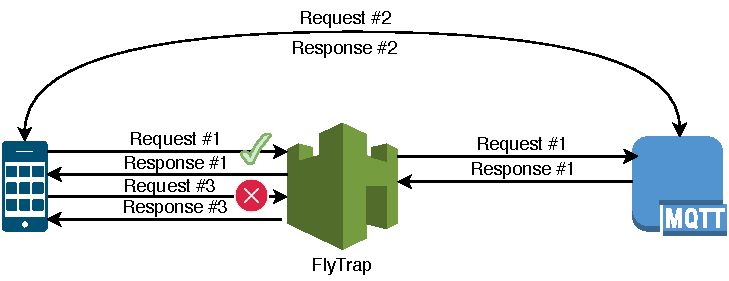
\includegraphics[width=0.8\textwidth]{tls}
    \caption{FlyTrap acting as a proxy.}
    \label{fig:tls}
\end{figure}

Figure \ref{fig:tls} demonstrates all 3 possibilities when a client attempts connection to a broker. In Request \#1, FlyTrap dissects the packet and confirm that the phone indeed can be allowed to access a specific topic and then start a bidirectional proxy with the MQTT broker, passing the TCP packets between them. Request \#2 shows that the same packet can be used with a vanilla MQTT Broker without FlyTrap, thus decoupling the client and secure proxy, as the former can be used without the need to change the latter. Finally, for the third request, it is found that the client cannot access the requested resource and is presented with a CONACK response, with the access denied flag set, terminating the connection. Though, in order to make such decisions, the proxy needs to inspect the contents of the packets.

Although TCP proxy is not be sufficient, as quickly as FlyTrap can tap into the connection, the same can be assumed for potential malicious actors, which could be listening on the flowing through packets. FlyTrap supports an extension to standard TCP - Transport Layer Security, or TLS for short, responsible for encrypting the TCP packets, significantly reducing the threat of man-in-the-middle attacks.

TLS sessions can be summarised in the following steps:
\begin{enumerate}
\item Initiate standard TCP session
\item ClientHello with client's cypher capabilities 
\item ServerHello and exchange of the cypher suite, along with the server's certificate
\item Key exchange and change of cypher spec
\item Encrypted session starts
\end{enumerate}

It is vital to point out, that due to step 3 requiring the server's certificate, FlyTrap needs to either obtain a copy of the broker's certificates or generate a new pair, ensuring that the connecting clients can trust it. Secure TLS connection remains optional, as it is understandable that sometimes enhanced security might cause undesirable performance losses (as found during the evaluation - see Section \ref{sec:tls_eval}) or the MQTT broker simply does not support TLS connections. As a result TLS usage with FlyTrap is configurable via command-line arguments. It is also possible to set TLS only on half of the journey, i.e. Client <-> FlyTrap is TLS-encrypted, but FlyTrap <-> MQTT Broker is not - and vice versa.

Moreover, for every new connection, a new thread (or, goroutine\footnote{Concept of threading defined by Golang. Goroutines can either be executed in the same address space or on a separate core, but it's all determined during runtime by Go runtime}) is spawned which has its own context and is separated from others, meaning that isolation between connections is maintained.

\subsubsection{Protecting from Brute-force Attacks}\label{sec:ddos}
Some of the failed attempts\footnote{Such as providing forged signature or connecting from prohibited country.} can result in a persistent log to the blockchain, which often resulusts in a cost - especially if FlyTrap is operating on a public blockchain. This introduces another threat, as malicious actors may attempt to drain the Framework of available funds by logging many operations in a short period. Distributed Denial of Service (DDoS) attacks can also occur and overload the server, which - depending on hardware - could only handle a limited number of simultaneous connections.

To combat those problems, the Framework tracks any failed authentication attempts in an internal dictionary, mapping IP address to the number of failed attempts. This dictionary then is looked up whenever a new connection is initiated. If it is, then the TCP link shuts down, and the client informed that it is currently blacklisted. Though to give the benefit of the doubt, there is a grace period of 2 prior failed attempts before a timed ban is applied. Whenever failed authentication occurs, the counter is increased by one - and if that count increases 3, the connection is terminated and dictionary updated with time 5 minutes in the future - that is the earliest time at which the given IP can attempt the connection again.
\subsection{Broker Layer}

This layer is where the communication with the actual MQTT Broker occurs. Typically, it would be desirable to place both FlyTrap and the broker (e.g. Mosquitto) on the same machine (or at least the same network) to minimise latency - though it is not necessary. Depending on the outcome of the authorisation from the Client Layer, every packet from the client is forwarded to the broker, and every packet from the broker sent back to the client. Since each connection is an individual thread (running on a separate port), it also maintains information such as originating (\& destination) address and port - and this information persists as long as the original connection Client <=> FlyTrap remains open - which is only terminated if the client times out, requests disconnection or for any reason authentication to FlyTrap fails.

Similar to the section discussing encrypted connection, FlyTrap is capable of either connecting with TLS-capable brokers or via plain TCP if desired (though keeping the security implications in mind, as everyone intercepting the connection would be able to read the payload).

\subsection{Blockchain Layer}
In this layer, communication with the Ethereum node occurs. As described in the architecture section, FlyTrap can either read or write new data onto the chain. FlyTrap should be allocated its own smart contract containing chain code capable of verifying connecting clients and relevant data structures. 
\subsubsection{Data Model}
The root of all communication with blockchain is a smart contract that contains all chain code responsible for retrieving and storing information required by FlyTrap. Each organisation or entity willing to use FlyTrap should configure and deploy a new contract, which would be tied to a singular owner (i.e., a private key). Ethereum's chain code execution can be limited to only a particular set of addresses, here most of the sensitive operations (such as adding new publishers or subscribers) are restricted to either an owner or payable ETH\footnote{Cryptocurrency used on Ethereum blockchains} (set by the owner) - if the requestor is not an owner.

Then, each contract contains a single variable called ``topics'' which is a mapping (dictionary structure in Solidity, a programming language for Ethereum) from a string (name of the topic) to structure ``Topic'' where the metadata can be located, such as control lists. Every person can create their own topic on the contract, of which they would become the owner. The contract's owner can also request ETH payment (in addition to the network fees) from any people looking to create a new topic. Figure~\ref{fig:uml_topic} shows all fields used in FlyTrap's chain code placed on the blockchain, to explain further the usage and purpose of each of the fields - with Figure~\ref{fig:uml_topic_example} showing example values:

\begin{figure}[h]
    \centering
    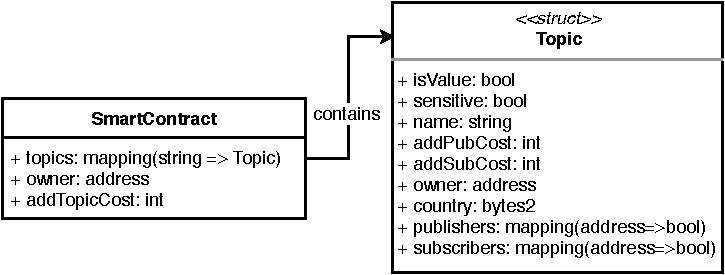
\includegraphics[width=0.9\textwidth]{uml_topic}
    \caption{Topic structure stored on blockchain.}
    \label{fig:uml_topic}
\end{figure}
\begin{figure}[h]
    \centering
    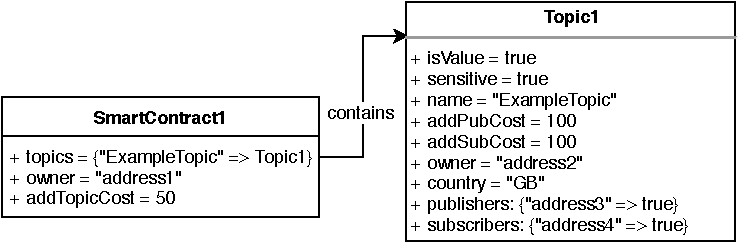
\includegraphics[width=0.9\textwidth]{uml_topic_example}
    \caption{Example values for a topic structure stored on blockchain. Note, "address(1|2|3|4)" refers to a public key, which is its own variable type in Solidity.}
    \label{fig:uml_topic_example}
\end{figure}

\begin{description}
    \item[isValue] - in Solidity, it is not possible to determine whether the given key exists in the mapping, as every value points to some arbitrary address space. An extra field helps to mitigate this issue, e.g. to avoid overwriting existing topics with new data.
    \item[sensitive] - a bool flag the marking given topic as sensitive which enhances it with extra data reporting functionality outlined in Section \ref{sec:reports}.
    \item[name] - a string storing the topic's name, as used by the clients on the broker. It is also used as the key in the topic's mapping.
    \item[addPubCost] - integer, fee (expressed in ETH) for adding a new publisher to the topic. See Section \ref{sec:monetization} for details.
    \item[addSubCost] - integer, similar as above, but for publishing.
    \item[owner] - ETH public address of the person that created this topic.
    \item[country] - 2-letter encoding of country to which access should be limited for all subscribers/publishers.
    \item[publishers] - mapping from the address of a person to a true/false bool value to determine whether the given public key can publish to this topic. It is a way of creating dynamic lists in Solidity, while maintaining $O(1)$ lookup time.
    \item[subscribers] - same as above, but for subscribers.
\end{description}

Apart from the structure show in Figure\ref{fig:uml_topic} holding information inside the contract, events are also utilised. Event is a special structure used in Solidity, which attaches itself to the transaction log. Meaning that it is possible to append information such as a user-specified reason or timestamps to all operations. This is then encoded in Application Binary Interface (ABI)\footnote{Encoding type used in Solidity: https://solidity.readthedocs.io/en/latest/abi-spec.html} JSON and sent along with the transaction. Though, it is also possible to emit empty events solely for logging purposes \citep{dannen2017introducing}.  Figure~\ref{fig:uml_event} outlines what each event consists of (with Figure~\ref{fig:uml_event_example} showing example usage):

\begin{figure}[h]
    \centering
    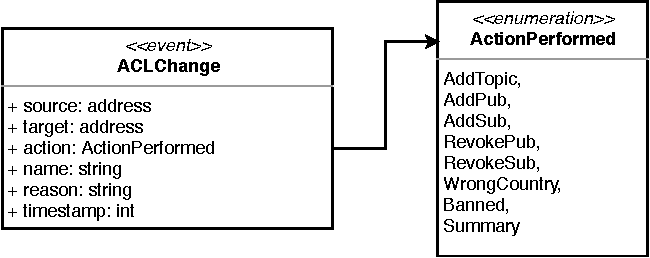
\includegraphics[width=0.8\textwidth]{uml_event}
    \caption{Event structure as stored in transaction log.}
    \label{fig:uml_event}
\end{figure}
\begin{figure}[h]
    \centering
    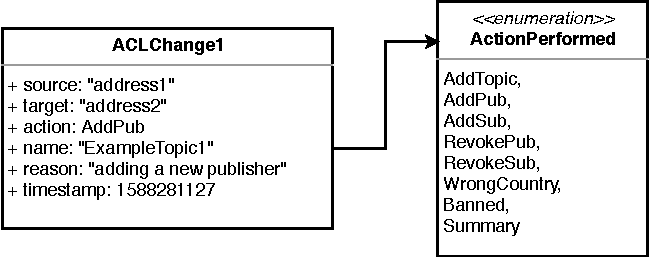
\includegraphics[width=0.8\textwidth]{uml_event_example}
    \caption{Example event log stored on Blockchain. It can be interpreted as follows: ``address1'' has added ``address2'' as a publisher to topic ``ExampleTopic1'' providing reason ``adding a new publisher''. This action modifies ``publishers'' mapping of ``ExampleTopic1'', by setting ``address2'' to true.}
    \label{fig:uml_event_example}
\end{figure}

\begin{description}
    \item[source] - ETH address of the entity that caused the log to emit. For example, for adding new topics or modifying a topic's properties (such as subscribers) it is the initiator's request. For system-caused logs (e.g. report summaries) it would be the contract's address.
    \item[target] - ETH address of the entity affected by the logged action. For example, for revoking publishers/subscribers, it would be the person that's being removed.
    \item[action] - enumeration, which defines the exact reason for emitting the log, this can be one of the following values:
    \begin{description}
        \item[AddTopic] - when a new topic is created on the contract.
        \item[AddPub] - when a new person is added as a publisher to the topic.
        \item[AddSub] - when a new person is added as a subscriber to the topic.
        \item[RevokePub] - when a person is removed from authorised publishers in the topic.
        \item[RevokeSub] - when a person is removed from authorised subscribers in the topic.
        \item[WrongCountry] - when a connection was attempted from an IP located in a country that is not permitted.
        \item[Banned] - when a person failed to authorise when connecting for three times in a row and was placed on a blacklist.
        \item[Summary] - system-generated log for sensitive topics (see \ref{sec:reports}).
    \end{description}
    \item[name] - string used to signify which topic was affected. If an action does not involve a topic, it contains the offending IP address used to make the request.
    \item[reason] - string provided either by the user or by the system to provide further context on the action (in particular, to answer questions given by GDPR, ``why was access provisioned?'').
    \item[timestamp] - UNIX timestamp (expressed as an integer) to determine when the transaction happened.
\end{description}
\subsubsection{Report Generation}\label{sec:reports}
For the most sensitive topics, it is possible to enhance security with extra measures and reporting. For every topic marked as sensitive, FlyTrap would maintain an in-memory list of all publishers or subscribers that have recently accessed the topic. Then, every specified period of time, a log is generated and placed on the blockchain that would outline all Ethereum public keys that have either published or subscribed to the given topic.

To put it in a perspective: if the reporting frequency is set at 30 minutes and the system is started at 12:00, then client A publishes to topic  X at 12:05, and client B publishes to topic X at 12:15, finally, at 12:30 a report would be generated and placed on the blockchain which would signify that both client A \& client B published to topic X between 12:00 and 12:30. The reports should be read as follows: In the past Y minutes\footnote{Where Y is the frequency}, the following public keys accessed the following sensitive topics. 

It is important to consider the implications of more and less frequent reporting - since every transaction placed on a blockchain with PoW\footnote{Proof-of-Work, see Section \ref{sec:pow} for details} consensus algorithm has an embedded gas price\footnote{Gas is a unit of work performed on Ethereum. The more complex the operation, the more gas is required, and thus more ETH currency is needed}, so the owner of the system would need to either accept the increased costs or decrease the reporting frequency. Of course, for PoA\footnote{Proof-of-Authority, see Section \ref{sec:poa} for details} algorithms, there is no gas cost, but still, the chain code's size would grow faster in case of more frequent reporting. However, with decreased frequency, the precision also falls, so if our reporting is set to 24hrs, now we can only determine the access history in daily windows (rather than 30min ones, as shown in the example above).
\subsubsection{Caching Operations}
Communicating with blockchain is a computationally expensive operation, and it is vital to ensure that it happens as rarely as possible in order to limit the latency caused by the security checks. Following the brute force approach, the Framework would issue a new request every time a connection starts - regardless whether it is part of a series of requests arriving in bulk. FlyTrap uses Ethereum as a de facto database layer, but at the same time aims to cache the operations in-memory, which can then be quickly accessed if repeated requests occur. For checking the permissions, whenever a new request is issued, the result is stored in a map with mutex lock (to avoid race conditions between different goroutines).

To avoid memory filling too quickly (and eventually reaching the capabilities of the server that is running the software), the mapping used for caching is erased every 24hrs or when the process is terminated/restarted - whichever happens first.

\subsubsection{Interacting with Blockchain}\label{sec:interact}
As FlyTrap aims to be deployed on a publicly available blockchain, anyone can interact with the data (as long as they pay the requested fee or identify with the relevant owner's private key). For administrative operations, a simple CLI is also included, which can be called directly (not necessarily through FlyTrap) to perform administrative tasks, such as adding new topics or modifying topic restrictions.

\subsubsection{Monetisation}\label{sec:monetization}
One of the biggest novelties of this project is the possibility to monetise the data published on MQTT brokers. When creating a new topic, a user interacting with the smart contract can specify a cost associated with adding publishers or subscribers to the blockchain. Once set, any arbitrary person can add their own public key to the ACL - granted they have enough funds to cover the fees. Then, those fees are transferred back to the topic creator - which can be spent or exchanged for fiat currency. The first revision of FlyTrap only allows fees to be set on changing ACLs\footnote{Disregarding how often the data is being accessed or how much data is published.} - for the future it might be interesting to also consider different tiers for different access frequencies. 

\subsection{Presentation Layer}
This layer provides a front-end for the data hosted on blockchain allowing users to inspect and interact with the stored information. Similarly to section \ref{sec:interact}, this could also be read through any of the publicly available front-ends used to interact with Ethereum transactions, but to provide a complete package, the project ships with a simple website which aims to satisfy the requirements stated in Chapter 3.
\subsubsection{Website}
The website does not allow for writing data to the blockchain (thus, does not require Ethereum wallet) which implies that all reading operations are free. The website's backend is loosly coupled with the Blockchain Layer, meaning that it permorms all of FlyTrap's free operations.

Due to how blockchain is designed, it is not possible to lookup a transaction from a specific time. Since it follows the design of a linked-list, lookup of all elements is required to find the requested date, thus resulting in the worst case complexity of $O(n)$, where $n$ is the amount of transactions in the smart contract. This might severely impact performance, especially as the chain grows, thus the web app keeps track of transaction hashes in 5-day intervals in-memory, updating as further requests are performed.

Front-ends operations are also restricted by a time-constraint, i.e. it would be possible to request reports generated between 1970-01-01 and 1971-01-01, warning the user that less restrictive constraints might result in longer lookup times.
